\chapter{Simulações Computacionais}\label{chapter:simulations}

Este capítulo apresenta a metodologia utilizada nas etapas de treinamento e teste do modelo GKR. Para isso, inicialmente são apresentados os conjuntos de dados utilizados para validação do desempenho. Para fins de comparação, são apresentados a metodologia e resultados dos seguintes métodos estado-da-arte: SVR, MLP e RBF.

A implementação do modelo GKR foi realizada utilizando a linguagem de programação Java\textsuperscript{TM} e a biblioteca de computação evolucionária ECJ (versão 23) \cite{luke2015}. Entretanto para o cômputo das aptidões dos indivíduos, bem como as implementações dos modelos SVR, MLP e RBF -- e quaisquer cálculos utilizando matrizes -- foi utilizado a plataforma Matlab\textsuperscript{TM}.

\section{Metodologia}
Como prova de conceito, inicialmente foram realizadas simulações com seis conjuntos de dados criados artificialmente. O primeiro conjunto, denominado Artificial I, é gerado a partir da função absoluto do seno dividido pelo padrão. O segundo conjunto, Artificial 2, é uma função do produto entre seno e cosseno. O terceiro conjunto, Artificial 3, é um semicírculo definido no intervalo $[-1,1]$. O quarto conjunto, Artificial 4, é um produto da tangente hiperbólica e do seno, gerando um formato parecido com a letra ``M''. O quinto conjunto, Artificial 5, é a função exponencial definida no intervalo $[-2,2]$. Por fim, o sexto conjunto, Artificial 6, é uma subtração de senos que gera um formato com curvas intermediárias na função seno padrão. Todos os conjuntos possuem um total de 1000 padrões e ruído gaussiano aditivo. A Tabela \ref{tab:art-datasets} apresenta um resumo dos conjuntos de dados e seus detalhes.

\begin{table}[H]
    \caption{Descrição dos problemas artificiais. $rand_i$ é uma amostra aleatória do ruído.}
    \label{tab:art-datasets}
    \begin{center}
            \begin{tabular}{ll@{\hskip 10pt}c@{\hskip 10pt}c} \hline\noalign{\smallskip}
            \textbf{Conjunto de Dados} & \textbf{Ruído} & \textbf{Função} & \textbf{Domínio} \\
            \noalign{\smallskip}
            \hline
            \noalign{\smallskip}
            Artificial 1 & $\rho(0, 0.08)$ & $y_i = |\sin(x_i)/x_i| + rand_i$ & $[-2\pi, 2\pi]$ \\
            Artificial 2 & $\rho(0, 0.2)$ & $y_i = \sin(x_i) \cos(1/x_i) + rand_i$ & $[-2\pi, 2\pi]$ \\
            Artificial 3 & $\rho(0, 0.1)$ & $y_i = \sqrt{1 - x_i^2} + rand_i$ & $[-1, 1]$ \\
            Artificial 4 & $\rho(0, 0.15)$ & $y_i = \tanh{(x_i)}\sin{(x_i)} + rand_i$ & $[-2\pi, 2\pi]$ \\
            Artificial 5 & $\rho(0, 0.25)$ & $y_i = \exp(x_i) + rand_i$ & $[-2, 2]$ \\
            Artificial 6 & $\rho(0, 0.5)$ & $y_i = \sin(6x_i) - 6\sin(x_i) + rand_i$ & $[-2\pi, 2\pi]$ \\
            \hline
        \end{tabular}
    \end{center}
    \begin{center}
        \makebox[\width]{Fonte: Autor.}
    \end{center}
\end{table}

Os problemas artificiais foram submetidos ao processo de aprendizado do algoritmo GKR, e uma análise qualitativa foi realizada com objetivo de examinar as superfícies de decisão obtidas, bem como os \textit{kernels} escolhidos para representação de cada problema. Os resultados destes experimentos são apresentados e discutidos na seção \ref{sec:results}.

Para avaliar o desempenho do modelo proposto neste trabalho em problemas do mundo real, foram realizadas simulações com conjuntos de dados disponíveis na coleção de problemas de regressão de \citeonline{torgo2018} e nos repositórios de aprendizado de máquinas da UCI \cite{dua2017} e \citeonline{statlib2018}. Os conjuntos de dados utilizados foram: \textit{Air Pollution}, \textit{Auto MPG}, \textit{Auto Price}, \textit{Boston Housing}, \textit{Computer Hardware}, \textit{Diabetes}, \textit{Servo Motor}, \textit{Sleep}, \textit{Spirituos Liquors}, \textit{Yacth Hydrodynamics} e \textit{Wisconsin Prognostic Breast Cancer}. A Tabela \ref{tab:real-datasets} apresenta o nome, abreviação, número de padrões e número de atributos de cada conjunto de dados utilizados nos experimentos.

\begin{table}[H]
    \caption{Conjuntos de dados reais utilizados neste trabalho.}
    \label{tab:real-datasets}
    \begin{center}
        \begin{tabular}{l@{\hskip 18pt}l@{\hskip 18pt}r@{\hskip 18pt}r}
            \hline\noalign{\smallskip}
            \textbf{Conjunto de dados} & \textbf{Abreviação} & \# \textbf{Padrões} & \# \textbf{Atributos}\\
            \noalign{\smallskip}
            \hline
            \noalign{\smallskip}
            \textit{Air Pollution} & APOL & 60 & 16 \\
            \textit{Auto MPG} & AMPG & 392 & 8 \\
            \textit{Auto Price} & APRI & 159 & 16 \\
            \textit{Boston Housing} & BHOU & 506 & 14 \\
            \textit{Computer Hardware} & CHAR & 209 & 7 \\
            \textit{Diabetes} & DIAB & 43 & 3 \\
            \textit{Servo Motor} & SERV & 167 & 5 \\
            \textit{Sleep} & SLEP & 51 & 8 \\
            \textit{Spirituous Liquors} & SPIR & 315 & 3 \\
            \textit{Stock Prices} & STPR & 950 & 16 \\
            \textit{Yacht Hydrodynamics} & YAHY & 308 & 7 \\
            \textit{Wisconsin Prognostic Breast Cancer} & WPBC & 194 & 33 \\
            \hline
        \end{tabular}
    \end{center}
    \begin{center}
        \makebox[\width]{Fonte: Autor.}
    \end{center}
\end{table}

Para realizar o treinamento do algoritmo GKR, é necessário que os conjuntos de dados passem por uma etapa de pré-processamento, chamada normalização. O objetivo desta etapa é fazer com que todos os atributos de um problema estejam na mesma escala, reduzindo o espaço de busca das soluções. Existem diversas técnicas de realizar a normalização tais como \textit{min-max} e \textit{z-score} (ou normalização de média zero) \cite{han2011}. Em todos os experimentos realizados neste trabalho foi utilizada a normalização \textit{min-max}, em que todos os valores de um atributo $f$ são subtraídos pelo valor mínimo deste atributo e dividido pela diferença entre os extremos (ou seja, $\max-\min$). Dessa forma, o valor normalizado de um atributo $f_i$ é obtido utilizando a seguinte equação

\begin{equation}
    \label{eq:ch4-1}
    \hat{f}_i = \frac{f_i - \min(f)}{\max(f) - \min(f)},
\end{equation}

\noindent em que $\min(f)$ é o valor mínimo do atributo $f$ e $\max(f)$, seu valor máximo. Assim, os valores normalizados $\hat{f}$ pertencem ao intervalo $[0, 1]$.

Uma característica intrínseca de modelos de AM é sua forte dependência no tocante às suas entradas; ou seja, o conjunto de treinamento escolhido, a dimensionalidade dos padrões e os hiperparâmetros\footnote{Parâmetros que não afetam o modo de funcionamento de um modelo, mas seu desempenho.} afetam diretamente seu desempenho. Por ser um modelo baseado em PG, o algoritmo GKR é formado por populações de indivíduos ao longo de um determinado número de gerações; uma vez que estes indivíduos são utilizados como componentes do modelo KRR (gerando a matriz de \textit{kernel}, $K$), o número de modelos obtidos através do KRR é igual ao número de indivíduos. Portanto, cada indivíduo deve ser avaliado como um modelo único de AM.

Cada indivíduo existente durante o processo de evolução representa uma função de \textit{kernel}, a qual possui um conjunto de parâmetros que afetam diretamente o poder de generalização que este fornece ao modelo KRR. %Parâmetros que influenciam no desempenho de um modelo de AM são chamados de hiperparâmetros.
Diversas técnicas foram propostas para encontrar o melhor conjunto de hiperparâmetros de um modelo de AM. A mais utilizada dentre elas é a combinação de uma busca em grade (do inglês, \textit{grid search}) com validação cruzada (do inglês, \textit{cross-validation}). Entretanto, uma vez que os hiperparâmetros são gerados por constantes efêmeras do conjunto de terminais, somente a validação cruzada é utilizada para avaliação de desempenho de cada indivíduo.

A ideia subjacente à validação cruzada encontra-se na divisão dos dados em uma ou mais partes, para estimação do risco de um algoritmo. Dessa forma, parte dos padrões são utilizados para o treinamento do algoritmo enquanto o restante é utilizado para estimar seu risco. Por fim, o algoritmo com menor risco é selecionado para construção do modelo final. As principais técnicas de validação cruzada são: \textit{holdout}, \textit{k-fold} e \textit{leave-one-out}. Neste trabalho foram utilizados apenas as duas primeiras técnicas.

Na técnica \textit{holdout}, o conjunto de dados é dividido em dois subconjuntos mutuamente excludentes: um para treinamento do algoritmo e obtenção do modelo, outro para teste e estimação do risco empírico (obtido através do cômputo do RMSE, equação \ref{ch3:eq29}). A avaliação da generalização de um determinado modelo é realizada utilizando o \textit{holdout} em sua formulação padrão (descrita acima), ilustrada na Figura \ref{fig:holdout}.

\begin{figure}[H]
    \caption{Uso do método \textit{holdout} para estimação do risco empírico.}
    \label{fig:holdout}
    \centering
    \hspace*{1.5cm}
    % 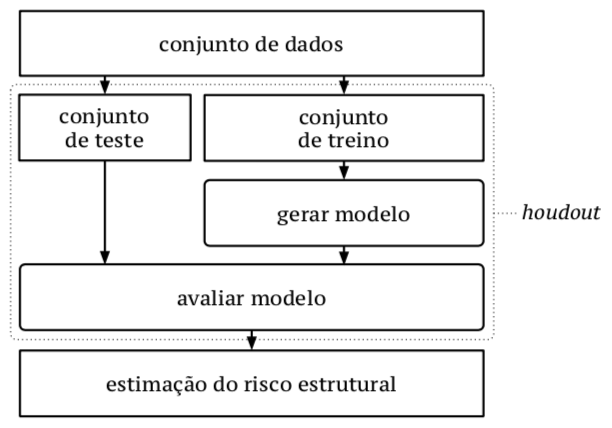
\includegraphics[width=.5\linewidth]{holdout.png}
    \begin{tikzpicture}[auto,
        block/.style = {rectangle, draw, fill=none, text width=8em, text centered, minimum height=2em}]
        % Place nodes
        \node [block, text width=15em] (dataset) {\scriptsize conjunto de dados};
        \node [block, node distance=1.8cm, below right of=dataset, xshift=0.15cm] (train) {\scriptsize conjunto de treinamento};
        \node [block, node distance=1.8cm, below left of=dataset, text width=6em, xshift=-0.6cm] (test) {\scriptsize conjunto de teste};
        \node [block, node distance=1.5cm, below of=train] (model) {\scriptsize gerar modelo};
        \node [block, node distance=4.25cm, text width=15em, below of=dataset] (evaluate) {\scriptsize avaliar modelo};
        \node [block, below of=evaluate, node distance=1.25cm, text width=15em] (risk) {\scriptsize estimação do risco estrutural};

        % Draw edges
        \draw[red, very thick, dotted, rounded corners] ($(test.north west)+(-0.2,0.2)$) rectangle ($(evaluate.south east)+(0.2,-0.2)$) node[text=black] at ($(model.east)+(1.2,0)$, 0) {\scriptsize \textit{holdout}};
        \path [line] ([xshift=14.2mm] dataset.south) -- (train.north);
        \path [line] ([xshift=-18.8mm] dataset.south) -- (test.north);
        \path [line] (train) -- (model);
        \path [line] (model.south) -- ([xshift=14.2mm] evaluate.north);
        \path [line] (test.south) -- ([xshift=-18.8mm] evaluate.north);
        \path [line] (evaluate) -- (risk);
    \end{tikzpicture}
    \begin{center}
        \makebox[\width]{Fonte: \citeonline{madson2017}.}
    \end{center}
\end{figure}

A técnica de validação cruzada \textit{k-fold} realiza uma divisão do conjunto total de dados em $k$ partes (subconjuntos) mutuamente excludentes de mesmo tamanho. Em seguida, um total de $k-1$ partes é utilizado no treinamento do algoritmo, enquanto a parte restante é utilizada para validação do modelo obtido. Este processo é realizado $k$ vezes, alternando de forma circular o $k$-ésimo conjunto utilizado para validação. Quando o processo é encerrado, computa-se o risco médio para os $k$ modelos, que é utilizado como estimação do risco estrutural. A Figura \ref{fig:k-fold} ilustra o processo descrito acima.

\begin{figure}[H]
    \caption{Uso do método \textit{k-fold} para estimação do risco empírico.}
    \label{fig:k-fold}
    \centering
    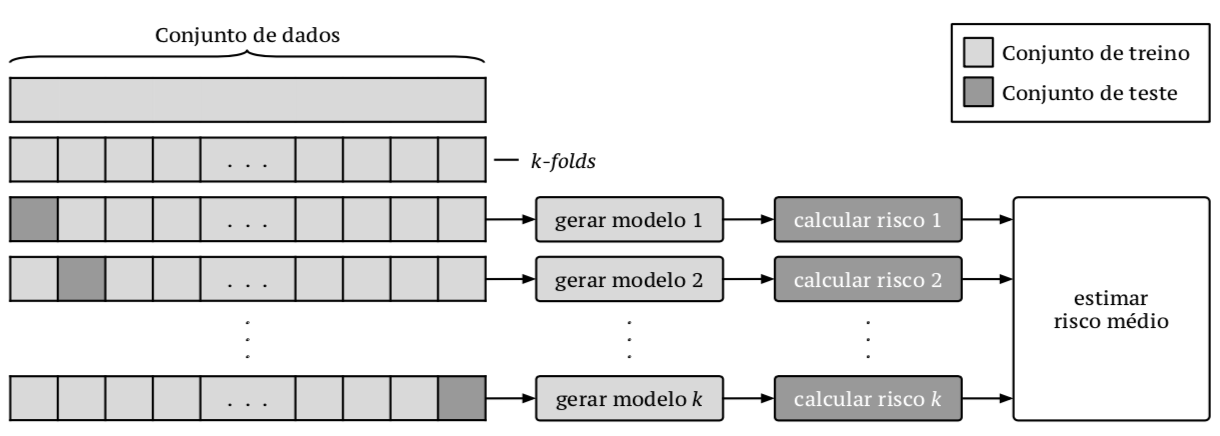
\includegraphics[width=\linewidth]{kfold.png}
    \begin{center}
        \makebox[\width]{Fonte: \citeonline{madson2017}.}
    \end{center}
\end{figure}

A realização de todos os experimentos deste trabalho utilizou uma combinação dos métodos \textit{holdout} e \textit{k-fold}. Primeiramente, o método \textit{holdout} realizou uma divisão onde 80\% dos dados foi utilizado para treinamento e os 20\% restantes para teste foi utilizado para estimação das métricas de desempenho, que para o caso específico de regressão são RMSE e tempo (total) médios. Em seguida, o método \textit{k-fold}, com 5 divisões ($k=5$), foi utilizado para definição da aptidão de cada indivíduo (\textit{kernel}), utilizando o conjunto de treinamento para tal divisão.

Existem ainda um conjunto de parâmetros relativos ao arcabouço de PG que precisa ser definido. A população inicial é criada utilizando o método \textit{ramped half-and-half} com faixa de profundidade $[2, 4]$. As probabilidades de uso dos operadores de cruzamento e mutação são 0.85 e 0.15, respectivamente. O método de seleção utilizado foi a seleção por torneio lexicográfico de tamanho 5. O tamanho da população foi definido em 30 indivíduos. Por fim, o número de gerações escolhido foi 30. A Tabela \ref{tab:pg-params} apresenta uma lista destes parâmetros e seus respectivos valores.

% Por último, o parâmetro de regularização foi fixado com valor $0.01$

\begin{table}[H]
    \caption{Resumo dos parâmetros utilizados nas realizações da PG.}
    \label{tab:pg-params}
    \begin{center}
        \begin{tabular}{l@{\hskip 18pt}l}
            \hline\noalign{\smallskip}
            \textbf{Parâmetro} & \textbf{Valor}\\
            \noalign{\smallskip}
            \hline
            \noalign{\smallskip}
            Número de gerações & 30 \\
            Tamanho da população & 30 \\
            Faixa de profundidade & $[2, 4]$ \\
            População inicial & \textit{ramped half-and-half} \\
            Método de seleção & \textit{lexicographic tournament} \\
            Tamanho do torneio & 5 \\
            Probabilidade de cruzamento & 0.85 \\
            Probabilidade de mutação & 0.15 \\
            \hline
        \end{tabular}
    \end{center}
    \begin{center}
        \makebox[\width]{Fonte: Autor.}
    \end{center}
\end{table}

\vspace*{-0.7cm}

Cada experimento foi realizado 30 vezes para cada par \textit{conjunto de dados/modelo} com base na seleção aleatória dos subconjuntos de treinamento e teste, com o parâmetro de regularização com valor fixo de $0.01$. As estimativas das métricas de avaliação foram definidas como uma média geral das 30 realizações.

\subsection{Comparação com modelos estado-da-arte}
Para fins de comparação de desempenho com o modelo proposto, são utilizados os seguintes modelos estado-da-arte: SVR, MLP e RBF. Especificamente para o SVR, foram utilizados os \textit{kernels} linear, polinomial e rbf. Para todos estes modelos, os hiperparâmetros foram obtidos utilizando uma modificação da metodologia do GKR: durante a validação cruzada de \textit{k-folds} é realizada uma busca em grade sobre uma faixa de valores dos hiperparâmetros. Para tornar a comparação mais justa, todos os modelos foram submetidos às mesmas divisões do método \textit{k-fold}, garantindo então que todos sejam submetidos às mesmas variações dos conjuntos de dados. O algoritmo de treinamento do SVR utilizado nos experimentos é o SMO \cite{platt1999}.

O hiperparâmetro do SVR com \textit{kernel} linear é apenas a constante de regularização \textit{C}, onde foi utilizado a faixa de valores em escala logarítmica $[10^{-3}, 10^3]$. Os outros \textit{kernels} (\textit{rbf} e polinomial) possuem dois hiperparâmetros, um deles sendo a constante $\gamma$ (com a mesma faixa de valores usada para o \textit{kernel} linear). Especificamente para o \textit{kernel} polinomial, foi utilizado a faixa de valores $[2, 4]$ para o grau do polinômio. Já para o SVR com \textit{kernel} rbf foi utilizada a faixa de valores em escala logarítmica $[10^{-3}, 10^3]$.

Para a rede neural MLP, o hiperparâmetro é o número de neurônios da camada oculta, em que a faixa de valores escolhida foi $[5, 25]$. O treinamento do MLP é realizado através do algoritmo de Levenberg-Marquardt \cite{hagan1994}. Já para a rede RBF \cite{powell1987}, há dois hiperparâmetros: o número de neurônios da camada oculta e a abertura da função gaussiana, $\sigma$. O número de neurônios da camada oculta tem faixa de valores em $[5, 25]$. A abertura da função gaussiana possui faixa de valores $[2^{-5}, 2^5]$.

\section{Resultados e Discussões} \label{sec:results}
Nesta seção são apresentados os resultados das simulações realizadas para avaliação da proposta deste trabalho. Para isso, o GKR, assim como SVR, MLP e RBF, são aplicados a diversos conjuntos de dados de natureza artificial e real, para problemas de regressão.

\subsection{Conjuntos de dados artificiais}
Para fins de análise do processo de treinamento, foram realizadas simulações utilizando conjuntos de dados artificiais de uma dimensão, uma vez que permite uma visualização das superfícies de decisão no plano cartesiano. Esta análise é importante, pois permite avaliar a capacidade de generalização dos modelos na representação dos dados, ou seja, a capacidade de aprendizado.

No primeiro grupo de experimentos deste trabalho foram utilizados apenas os seguintes modelos: GKR, MLP, RBF e SVR/RBF\footnote{É comum na literatura utilizar a nomenclatura \textit{regressor/algoritmo/kernel}; entretanto, como o algoritmo utilizado em todos os experimentos neste trabalho foi o SMO, a nomenclatura torna-se \textit{regressor/kernel}.}. Isso pode ser justificado pela pouca capacidade de generalização que os modelos SVR/LIN e SVR/POL apresentaram durante as simulações computacionais.

Na Figura \ref{fig:results-real-datasets} são apresentados os resultados obtidos para os seis conjuntos de dados artificiais. %A análise dos gráficos pode ser dividida em dois grupos: (\textit{i}) para funções com muitas 
Ao analisar os gráficos, percebe-se que os modelos GKR e SVR/RBF possuem superfícies bastante semelhantes, conseguindo representar bem os dados. Entre as redes neurais, a MLP é a mais eficiente na generalização dos dados, gerando superfícies mais flexíveis. Já a rede RBF não consegue obter o mesmo poder de generalização que a MLP, pois suas superfícies de decisão sempre seguem o formato da função gaussiana (formato de ``sino''). Nas Figuras \ref{fig:results-real-datasets-3} e \ref{fig:results-real-datasets-5}, entretanto, a rede RBF consegue uma boa representação, uma vez que o domínio de ambas as funções apresentam um formato parecido com partes da função gaussiana.

\begin{figure}[H]
    \caption{Superfícies de decisão geradas pelos modelos GKR, RBF, SVR/RBF e MLP para os conjuntos de dados artificiais.}
    \label{fig:results-real-datasets}
    \begin{subfigure}[b]{0.5\linewidth}
        \centering
        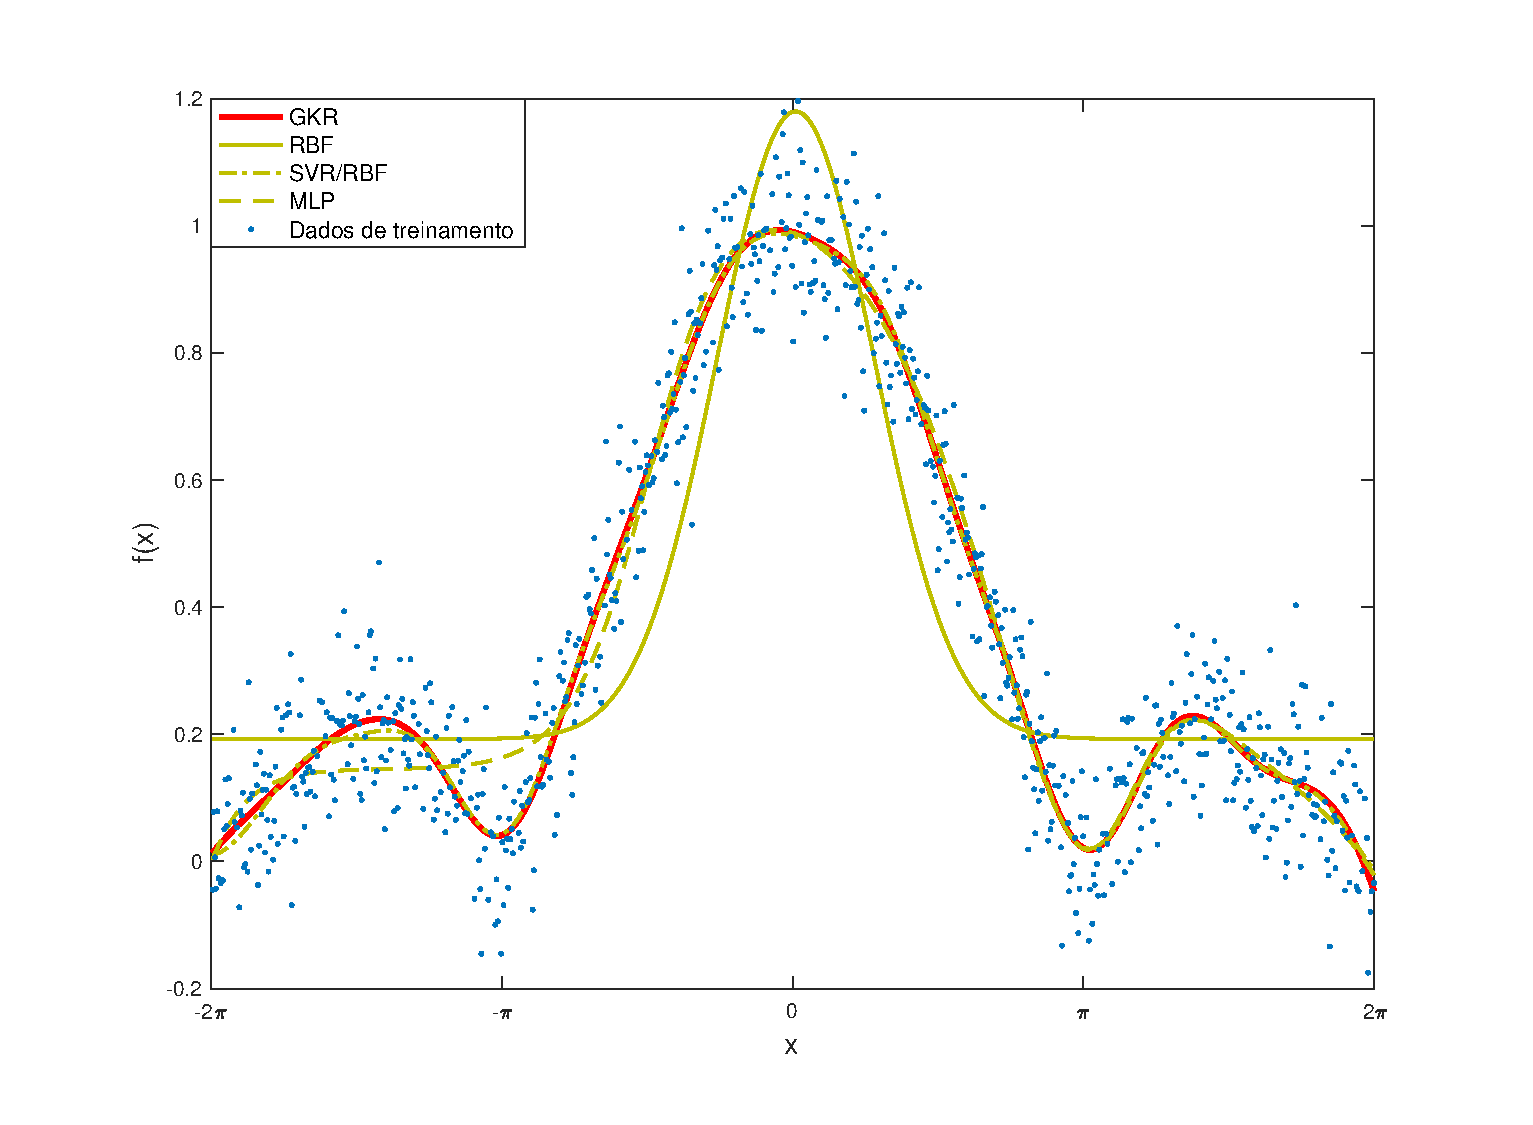
\includegraphics[width=\linewidth]{chapter4/art1.eps}
        \caption{Artificial 1} 
        \label{fig:results-real-datasets-1}
    \end{subfigure}%%
    \begin{subfigure}[b]{0.5\linewidth}
        \centering
        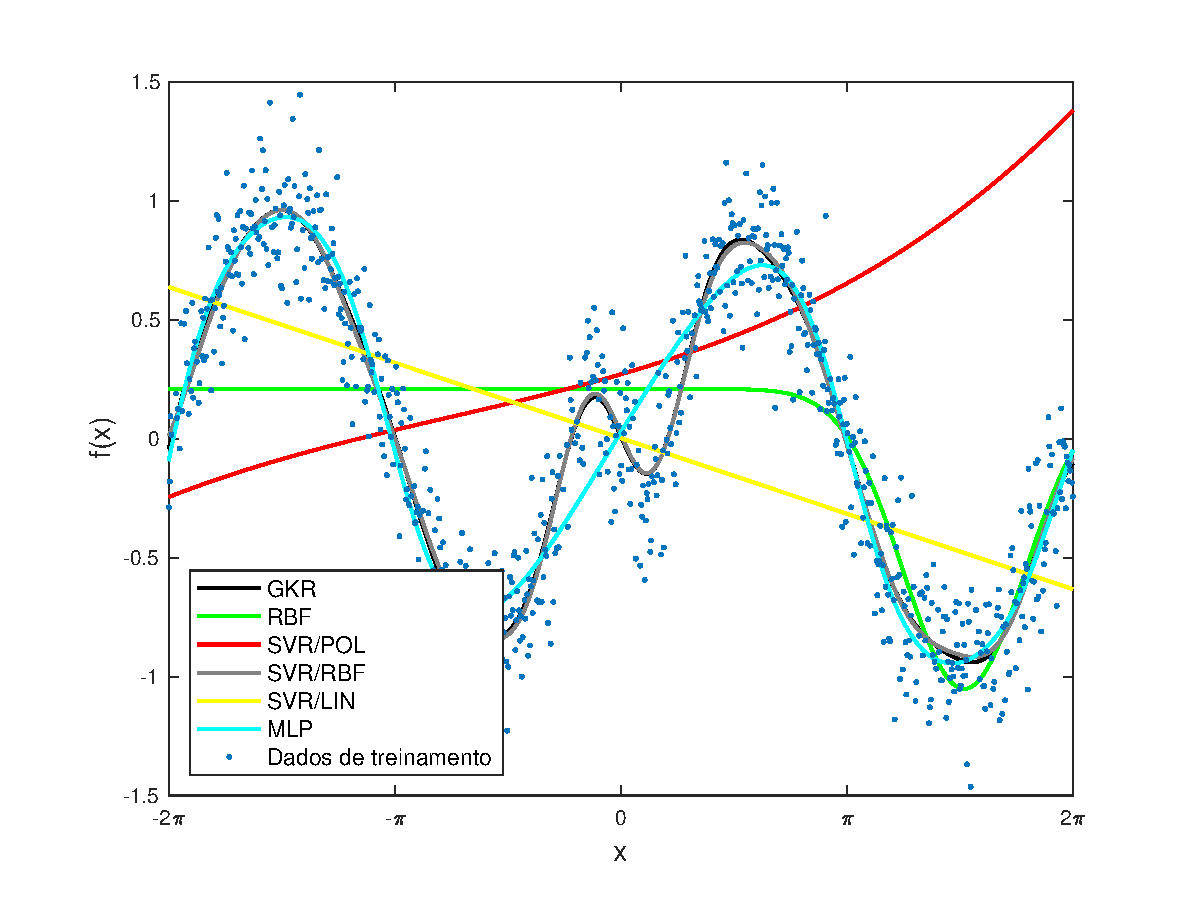
\includegraphics[width=\linewidth]{chapter4/art2.eps}
        \caption{Artificial 2}
        \label{fig:results-real-datasets-2}
    \end{subfigure}
    \begin{subfigure}[b]{0.5\linewidth}
        \centering
        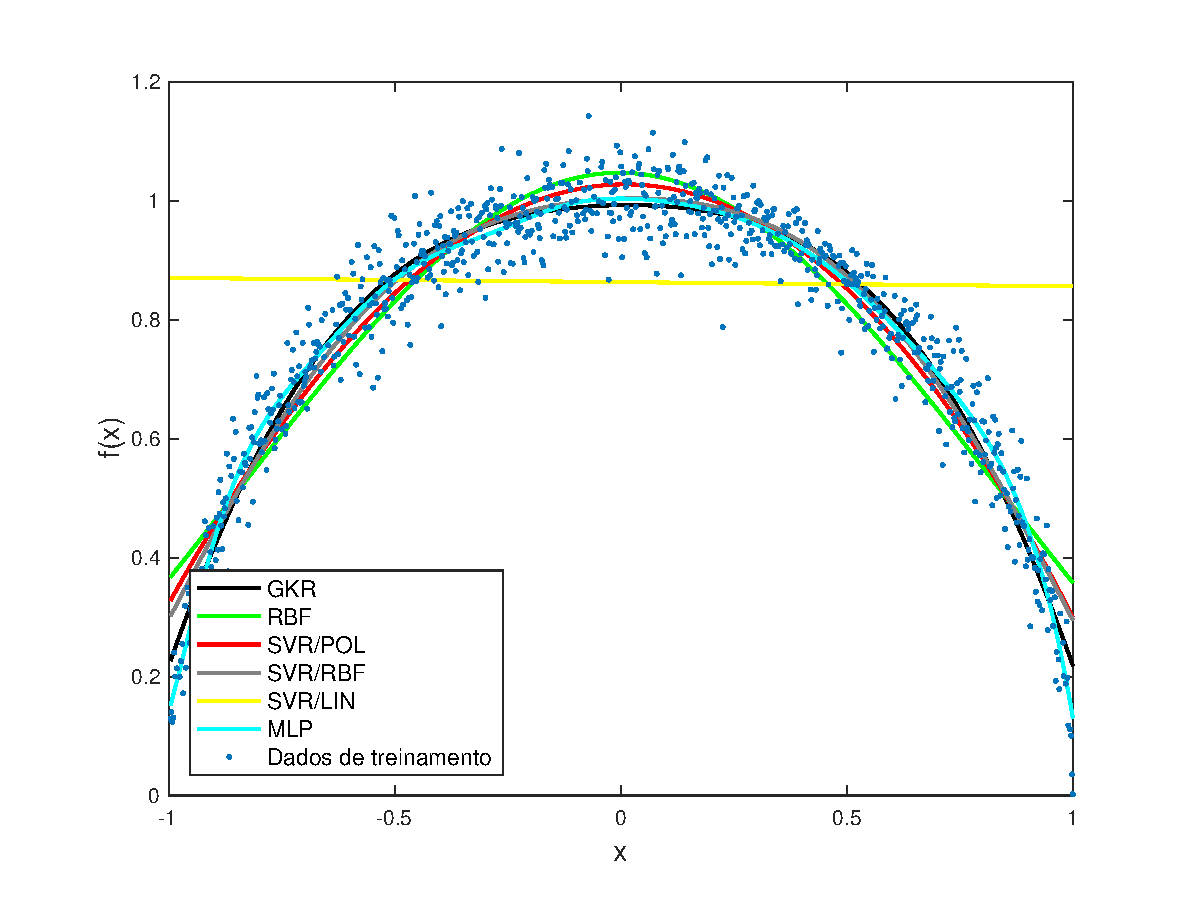
\includegraphics[width=\linewidth]{chapter4/art3.eps}
        \caption{Artificial 3}
        \label{fig:results-real-datasets-3}
    \end{subfigure}%%
    \begin{subfigure}[b]{0.5\linewidth}
        \centering
        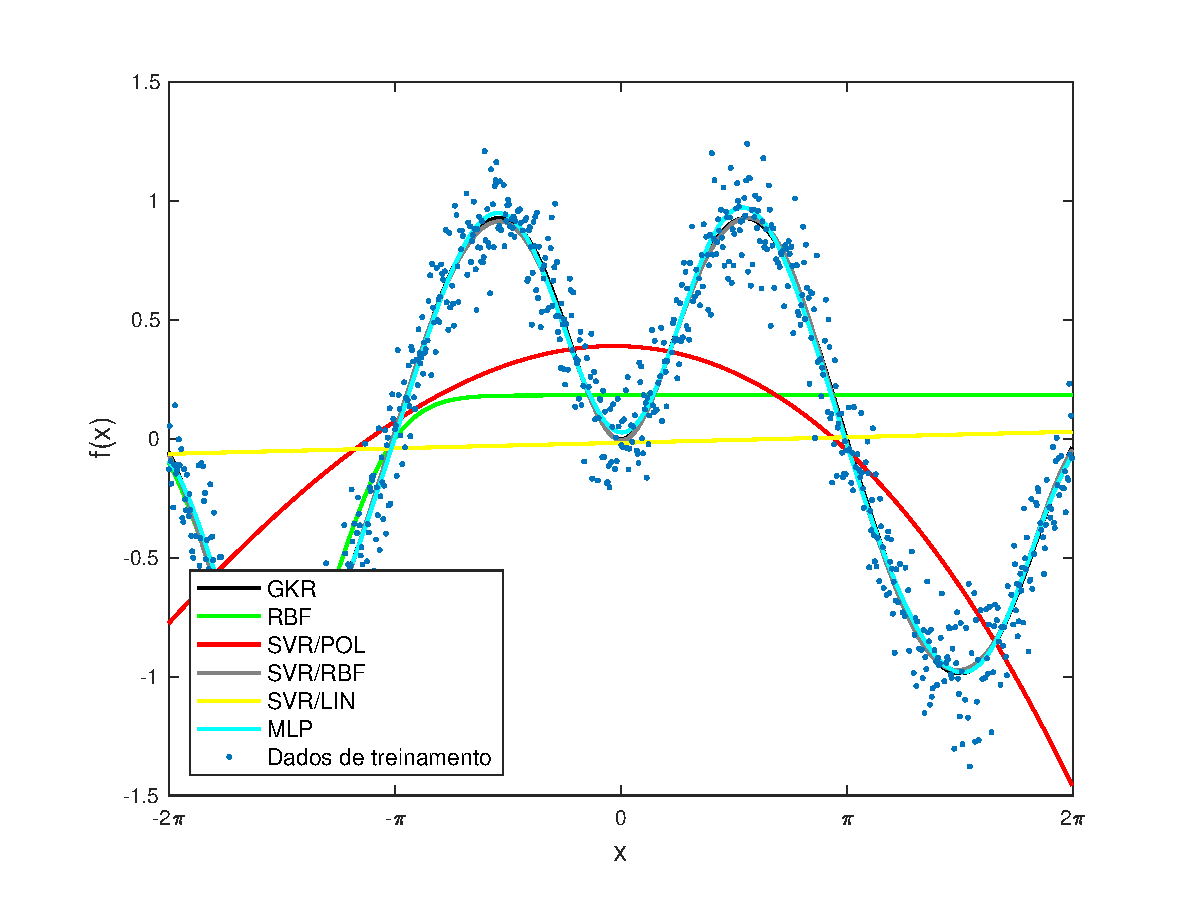
\includegraphics[width=\linewidth]{chapter4/art4.eps}
        \caption{Artificial 4}
        \label{fig:results-real-datasets-4}
    \end{subfigure}
    \begin{subfigure}[b]{0.5\linewidth}
        \centering
        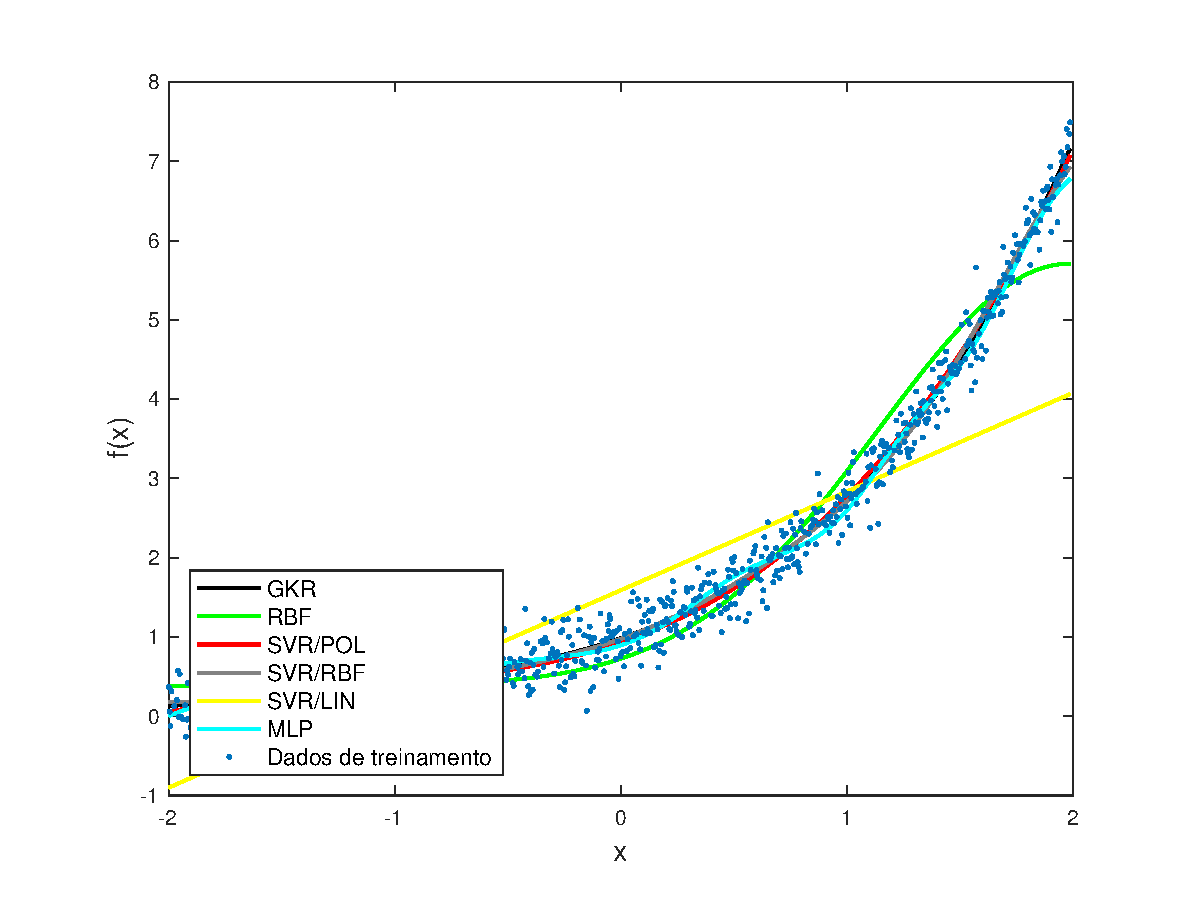
\includegraphics[width=\linewidth]{chapter4/art5.eps}
        \caption{Artificial 5}
        \label{fig:results-real-datasets-5}
    \end{subfigure}%%
    \begin{subfigure}[b]{0.5\linewidth}
        \centering
        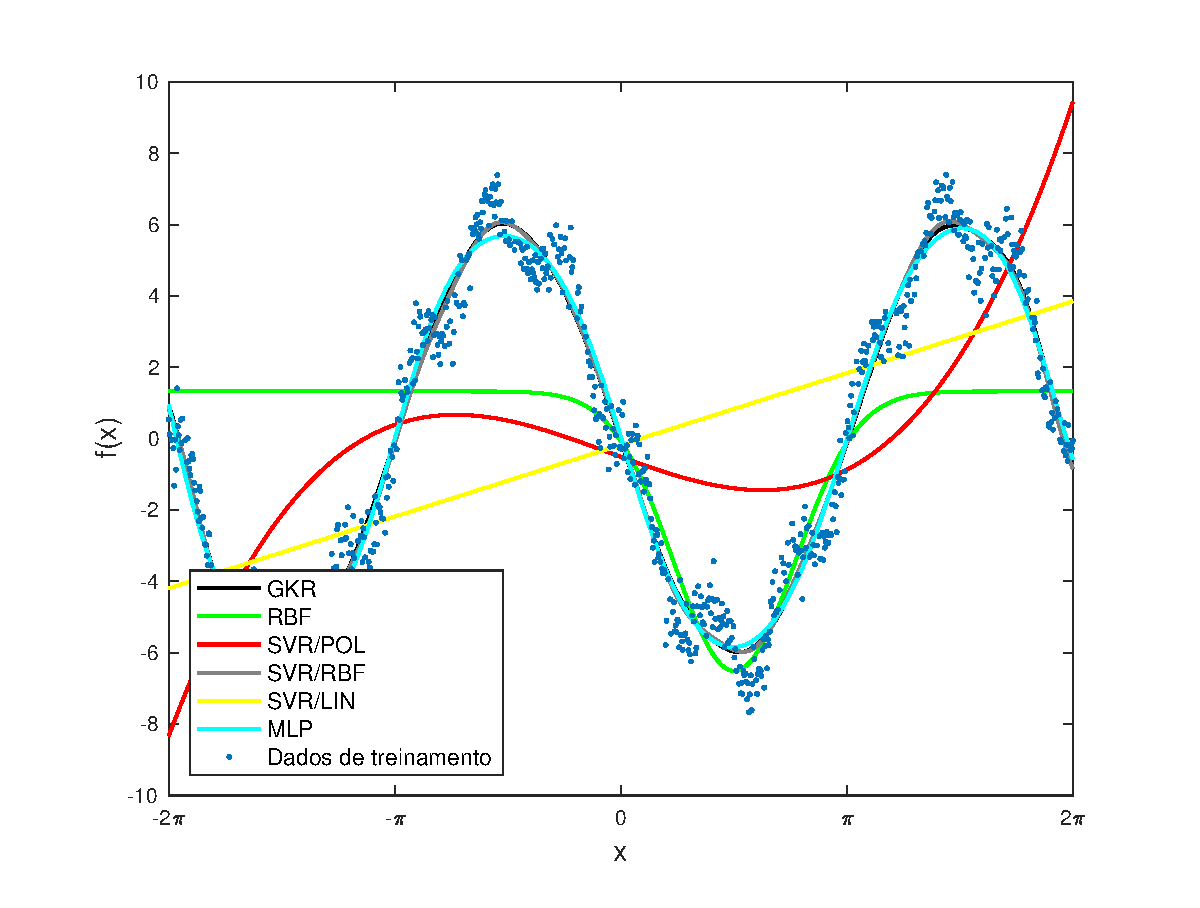
\includegraphics[width=\linewidth]{chapter4/art6.eps}
        \caption{Artificial 6}
        \label{fig:results-real-datasets-6}
    \end{subfigure} 
    \centering \makebox[\width]{Fonte: Autor.}
\end{figure}

\subsection{Conjuntos de dados reais}
O segundo grupo de experimentos tem como finalidade avaliar o desempenho do modelo GKR em problemas do mundo real, e compará-lo com o desempenho de modelos estado-da-arte. Para tal, as seguintes métricas serão analisadas: (\textit{i}) o desempenho das funções de \textit{kernel} será analisado através do valor de aptidão médio ao longo das gerações; (\textit{ii}) RMSE (média e desvio padrão); (\textit{iii}) tempo total (treinamento e teste) médio.

As Figuras \ref{fig:results-fitbygen1} e \ref{fig:results-fitbygen2} apresentam os resultados relativos aos conjuntos de dados reais. De modo geral, ao analisar ambas as figuras, percebe-se que a capacidade de representação dos dados vai se tornando cada vez melhor ao longo do processo de evolução. A partir disso pode-se confirmar que o algoritmo GKR consegue realizar a evolução das funções de \textit{kernel} de forma eficiente.

Um fator importante que precisa ser ressaltado é a influência que a natureza estocástica da PG exerce nos valores médios de aptidão a cada geração. De acordo com \citeonline{poli2008}, o processo de aprendizado de um sistema baseado em PG ocorre nas primeiras gerações\footnote{Os autores ainda afirmam que este é um dos motivos de que, de modo geral, o número de gerações de uma realização de PG é tipicamente inferior ou igual a 50.}. Portanto, é comum encontrar partes dos melhores indivíduos das primeiras gerações ao longo do processo de evolução. Portanto, a partir do crescimento do valor de aptidão médio ao longo das gerações, percebe-se que as funções de \textit{kernel} são candidatas equivalentes à solução ideal de cada problema (embora o modo em que a PG chega à essas funções é estocástico). Para a grande parte dos problemas, são poucos os decaimentos do valor de aptidão médio durante o processo de evolução. Entretanto, para problemas tais como \textit{Auto MPG}, \textit{Diabetes} e \textit{Servo Moto} há uma variação maior no valor de aptidão médio. Embora não seja um fator que chegue a causar descrédito ao GKR, pois o valor de aptidão médio permanece em faixas muito estritas (com mudanças na terceira casa decimal), serve para perceber duas situações: (\textit{i}) o conjunto de dados pode não representar bem o problema (ou seja, o problema pode sofrer de mal-condicionamento); (\textit{ii}) as funções de \textit{kernel} geradas durantes as realizações acabam não sendo candidatas equivalentes à solução do problema, o que acarreta no decaimento da aptidão média.

Para analisar a variabilidade do valor de aptidão média, pode ser realiza uma análise sobre a Tabela \ref{tab:results-rmse}. De modo geral, para todas os problemas reais utilizados neste trabalho, o desvio padrão dos modelos de regressão foi baixo -- com exceção da rede RBF, que para os problemas \textit{Diabetes} e \textit{Sleep}, obteve desvios padrões muito grandes. O fato de o RMSE não possuir muita variabilidade ao longo das 30 realizações permite inferir que o modelo GKR, assim como os modelos estado-da-arte, possui uma robustez grande a diversos problemas de regressão. Outro ponto a ser destacado é a capacidade de gerar diferentes funções de \textit{kernel} que conseguem adaptar-se à aleatoriedade dos conjuntos de treinamento e da própria natureza da PG; este fato permite inferir que o GKR consegue representar bem os dados que são apresentados a ele e construir \textit{kernels} adequados para cada situação.

Também é válido analisar o custo computacional e o tempo total necessário para realização dos modelos. Como era esperado (e já discutido brevemente no Capítulo \ref{chapter:kernel-methods}), o custo computacional do modelo KRR é da ordem $\mathcal{O}(n^3 + n^2p)$, onde $n$ é o número de padrões do conjunto e $p$ é a dimensionalidade dos padrões. Em conjunto com o arcabouço de PG, o tempo médio dispendido para treinamento e teste foi muito alto (inclusive maior que todos os modelos estado-da-arte). Porém, a justificativa para tais custos reside na validação cruzada de \textit{k-folds} que é realizada para cada indivíduo de cada população ao longo das gerações. Dessa forma, é de se esperar que o tempo necessário seja maior que dos outros modelos utilizados neste trabalho.

% Por fim, é feito uma análise entre os modelos SVR e KRR. Modelos como o SVR (e SVMs, de modo geral), advém da teoria do aprendizado estatístico. Uma característica importante do SVR é que ele consegue minimizar uma combinação do risco empírico e um termo de regularização responsável pela suavização da solução \cite{daniel2017}. O KRR possui uma formulação mais simples que o SVR. A principal diferença encontradas são a função de perda (\textit{ridge} para o KRR, \textit{\epsilon-insensitive} para o SVR)

\begin{figure}[H]
    \caption{Gráficos dos valores de aptidão médios ao longo das gerações (Parte 1).}
    \label{fig:results-fitbygen1}
    \begin{subfigure}[b]{0.5\linewidth}
        \centering
        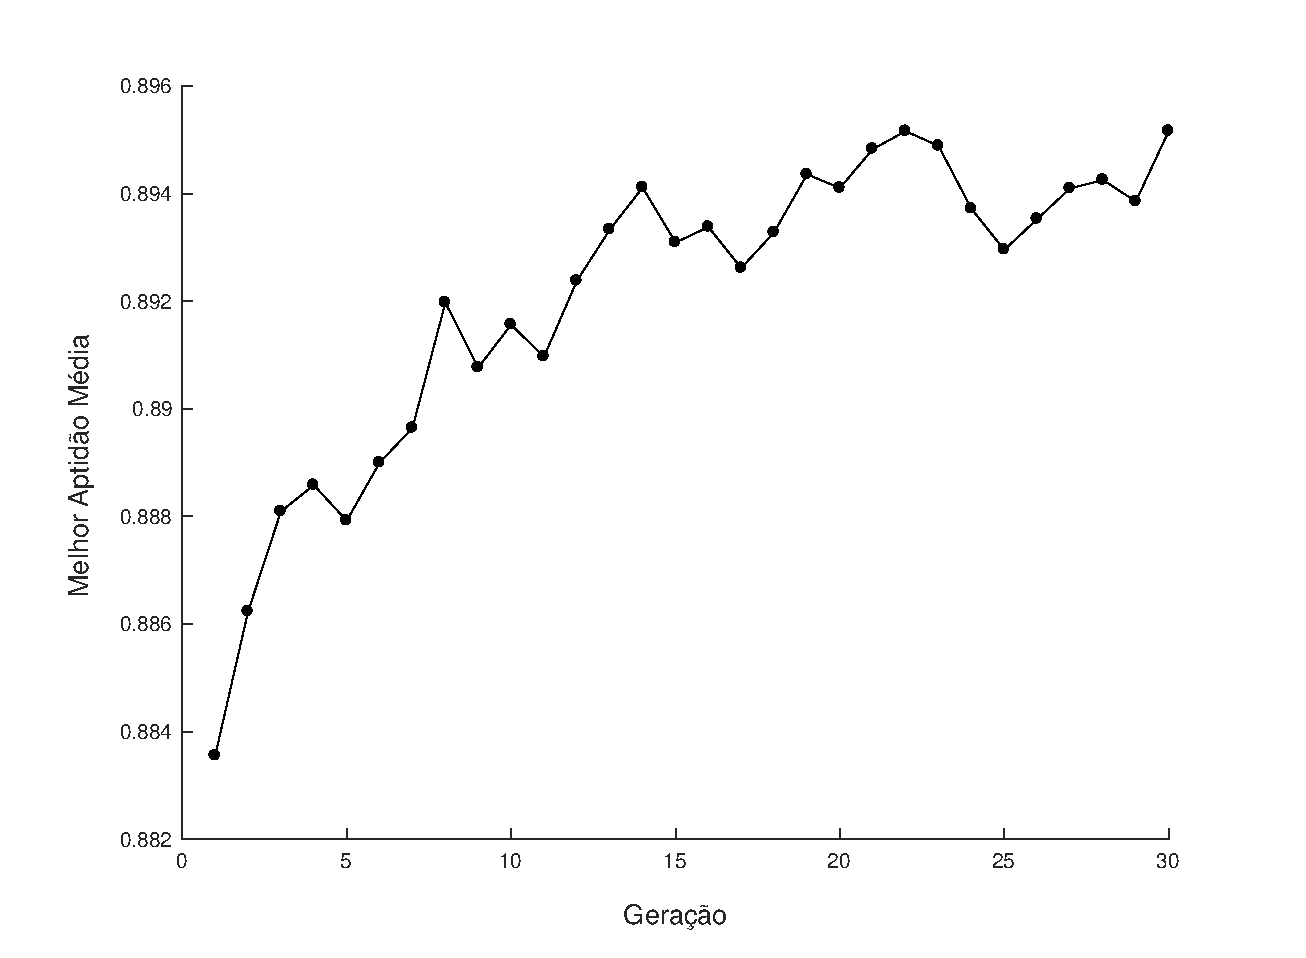
\includegraphics[width=\linewidth]{chapter4/air-pollution.eps}
        \caption{\textit{Air Pollution}} 
        \label{fig7:a}
    \end{subfigure}%%
    \begin{subfigure}[b]{0.5\linewidth}
        \centering
        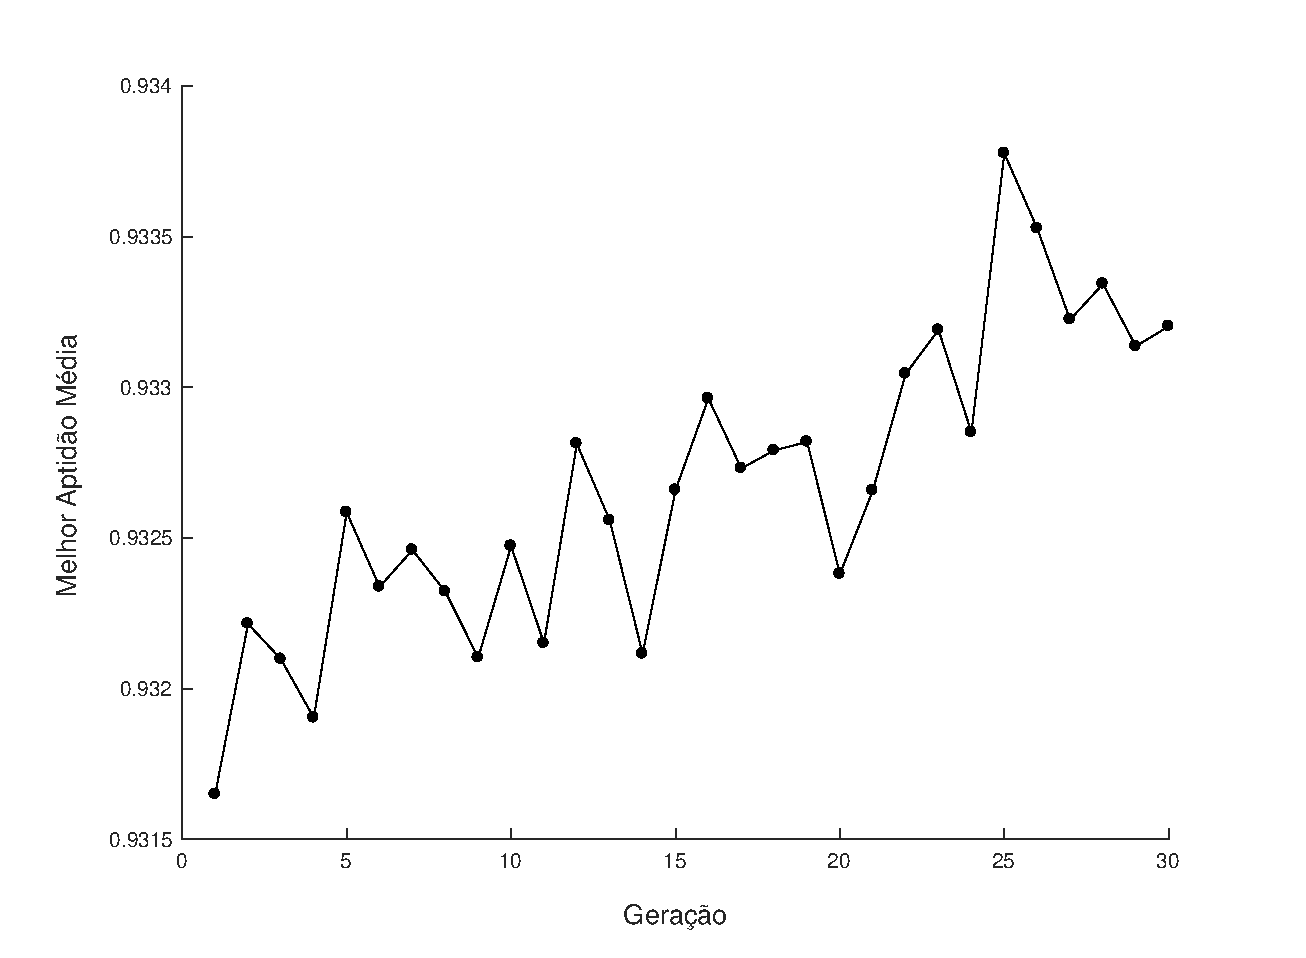
\includegraphics[width=\linewidth]{chapter4/auto-mpg.eps}
        \caption{\textit{Auto MPG}}
        \label{fig7:b}
    \end{subfigure}
    \begin{subfigure}[b]{0.5\linewidth}
        \centering
        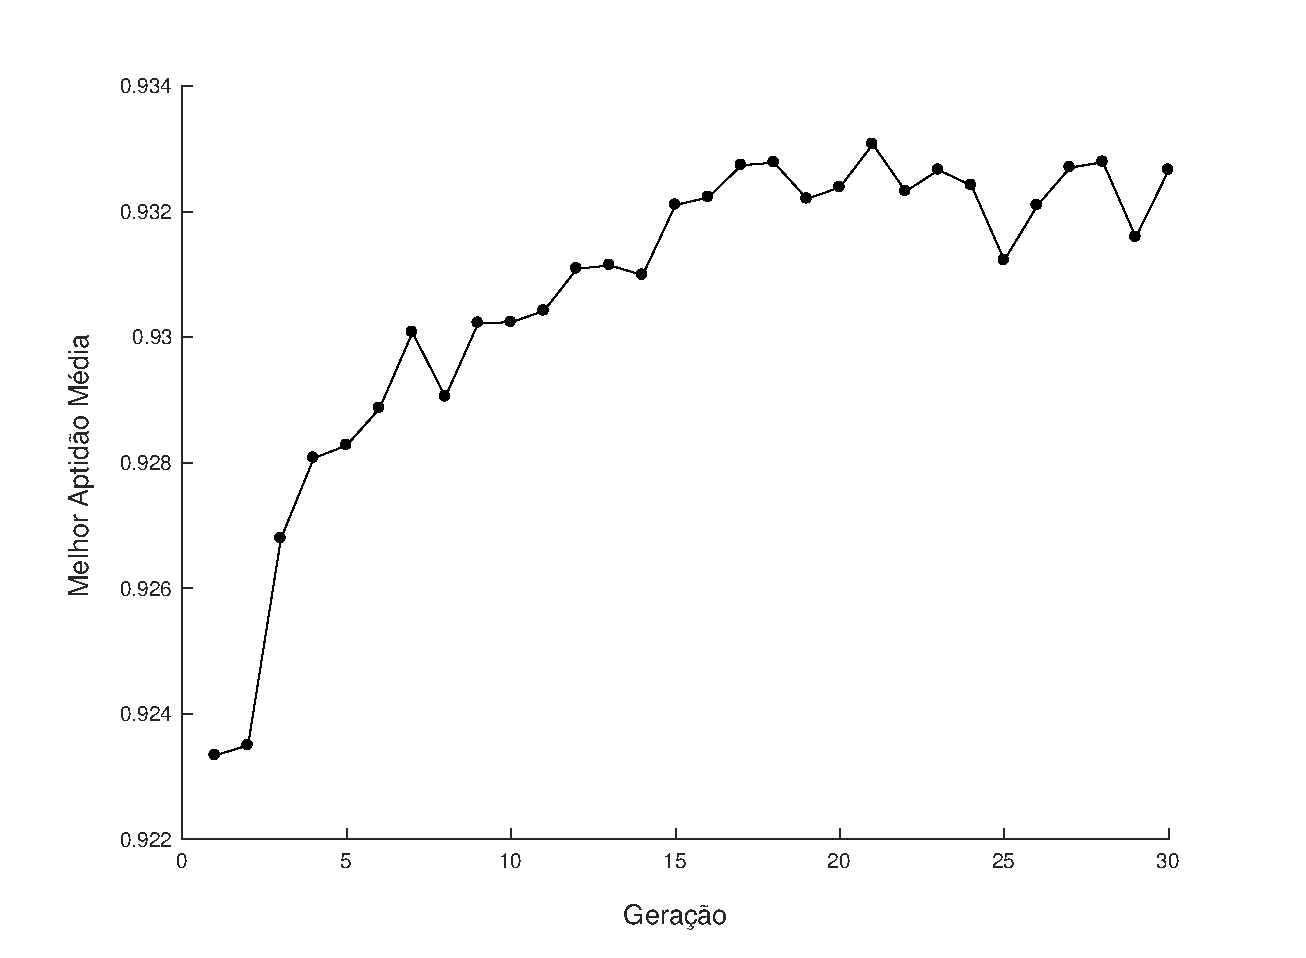
\includegraphics[width=\linewidth]{chapter4/auto-price.eps}
        \caption{\textit{Auto Price}}
        \label{fig7:c}
    \end{subfigure}%%
    \begin{subfigure}[b]{0.5\linewidth}
        \centering
        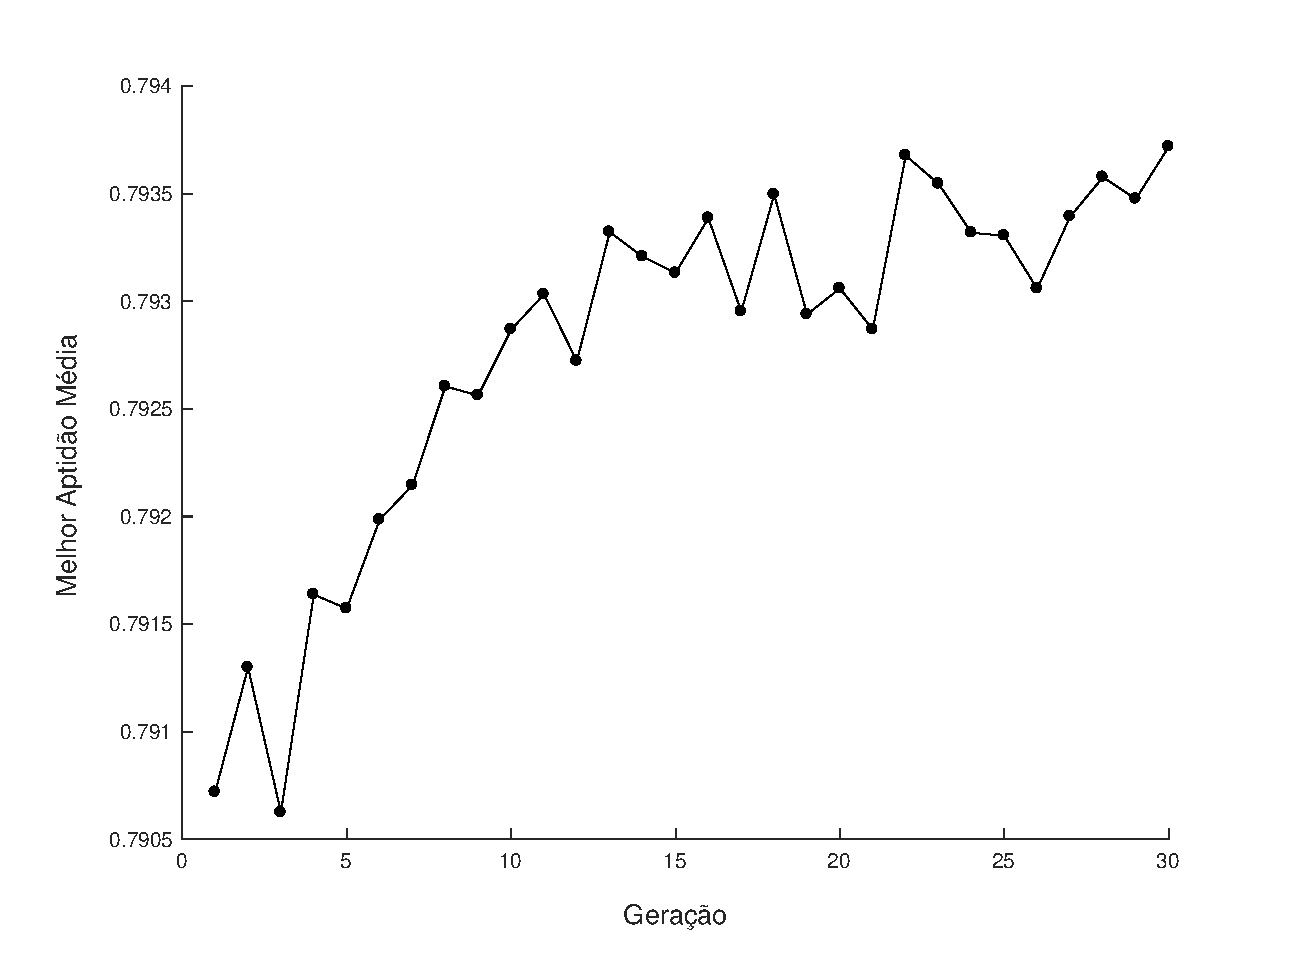
\includegraphics[width=\linewidth]{chapter4/breast-cancer.eps}
        \caption{\textit{Wisconsin Prognostic Breast Cancer}}
        \label{fig7:d}
    \end{subfigure}
    \begin{subfigure}[b]{0.5\linewidth}
        \centering
        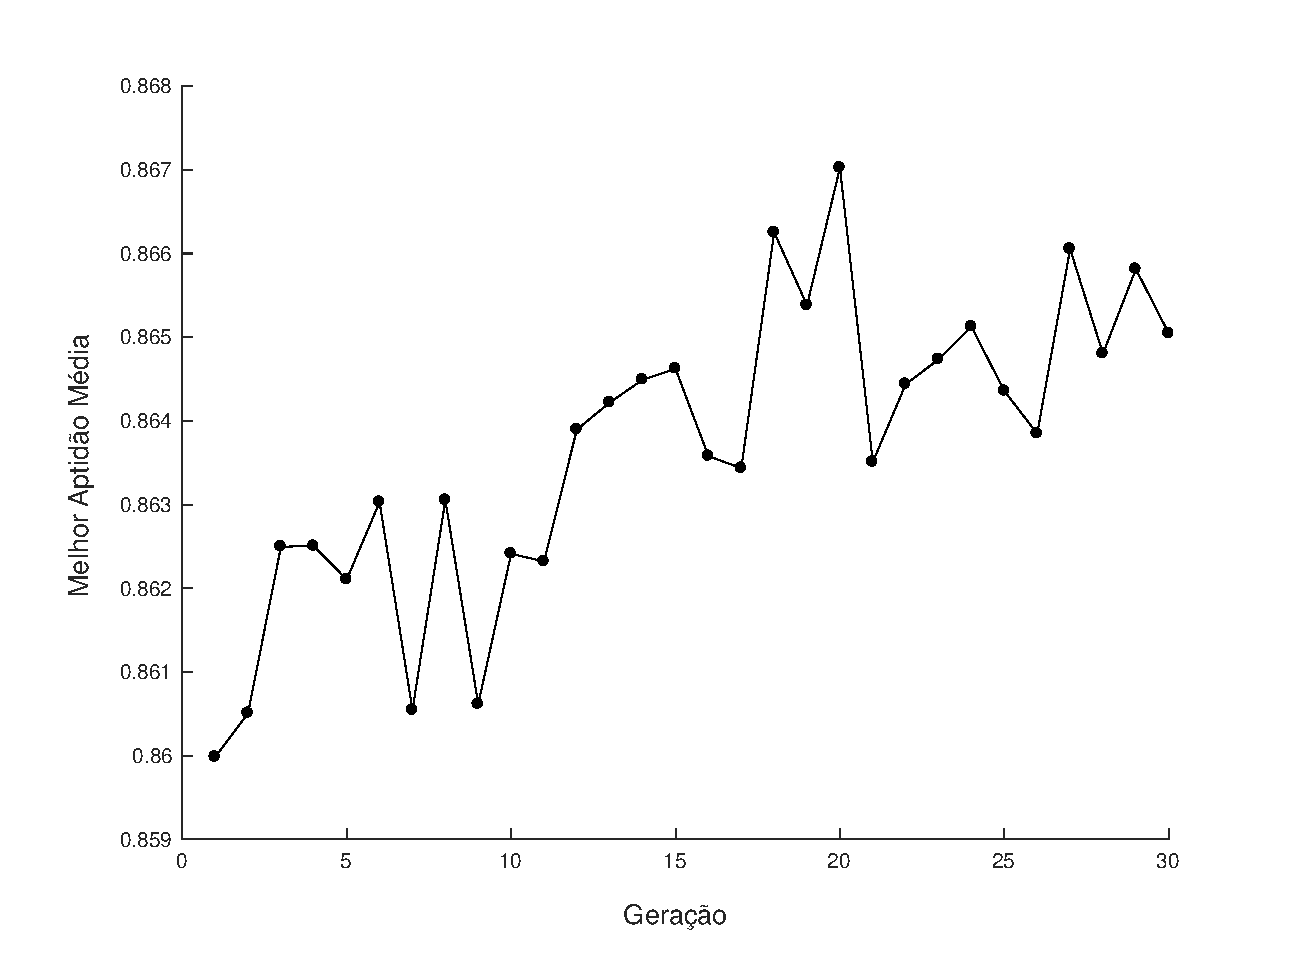
\includegraphics[width=\linewidth]{chapter4/diabetes.eps}
        \caption{\textit{Diabetes}}
        \label{fig7:e}
    \end{subfigure}%%
    \begin{subfigure}[b]{0.5\linewidth}
        \centering
        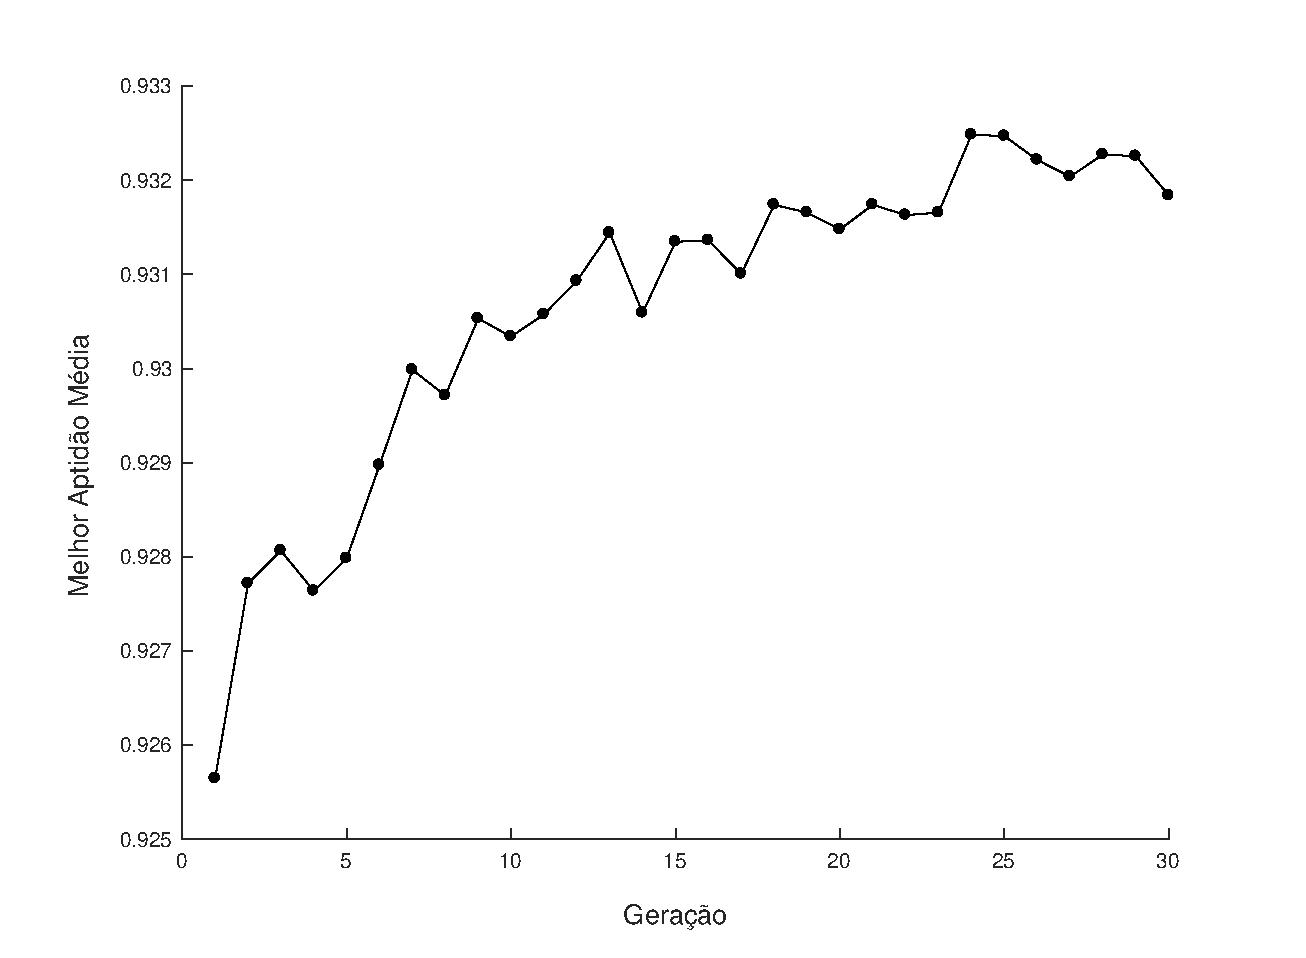
\includegraphics[width=\linewidth]{chapter4/housing.eps}
        \caption{\textit{Boston Housing}}
        \label{fig7:f} 
    \end{subfigure} 
    \centering \makebox[\width]{Fonte: Autor.}
\end{figure}
\begin{figure}[H]
    \caption{Gráficos dos valores de aptidão médios ao longo das gerações (Parte 2).}
    \label{fig:results-fitbygen2}
    \begin{subfigure}[b]{0.5\linewidth}
        \centering
        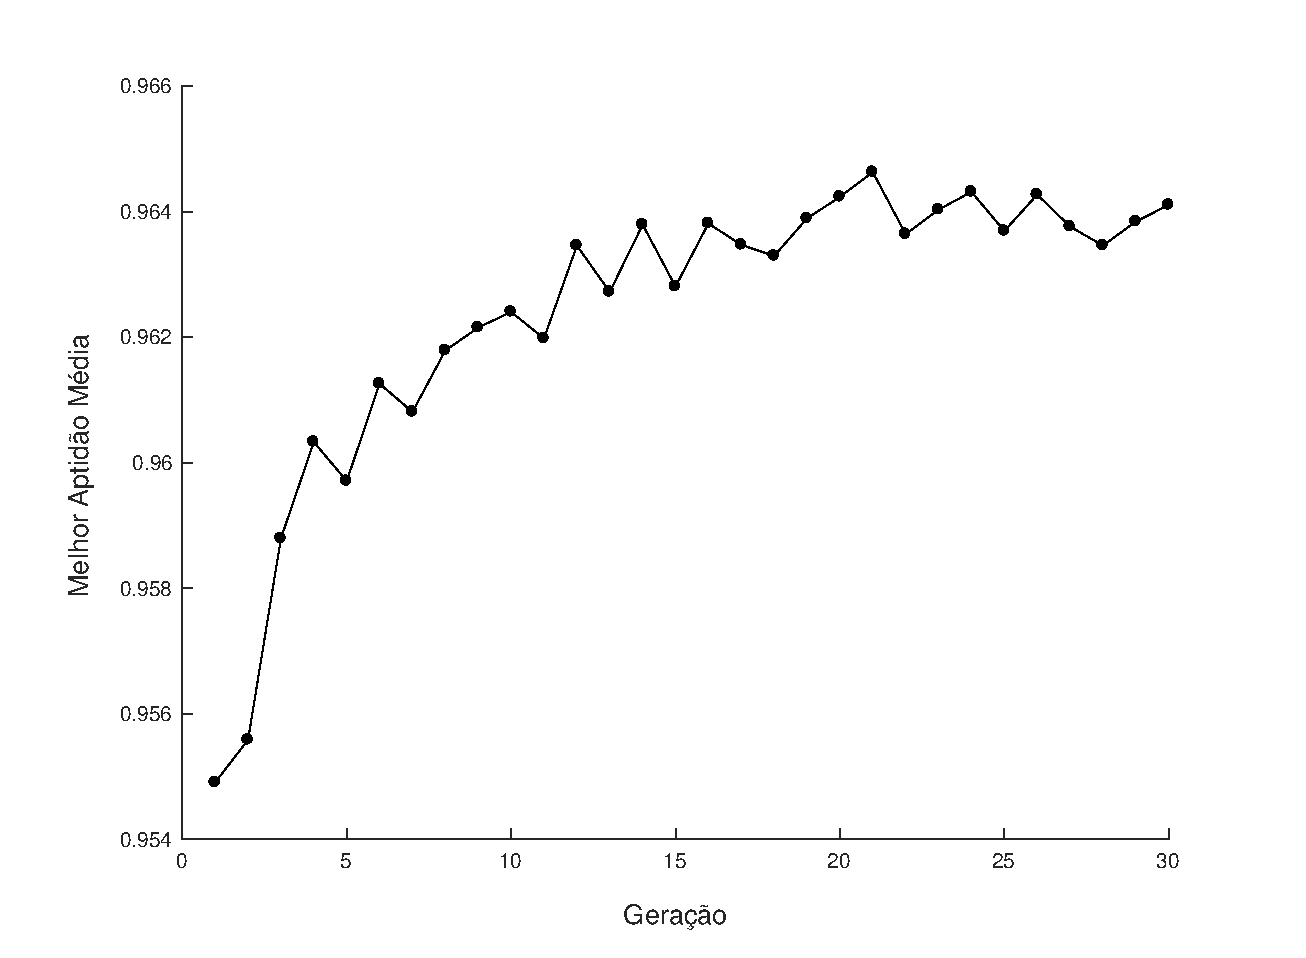
\includegraphics[width=\linewidth]{chapter4/machine-cpu.eps}
        \caption{\textit{Computer Hardware}} 
        \label{fig8:a}
    \end{subfigure}%%
    \begin{subfigure}[b]{0.5\linewidth}
        \centering
        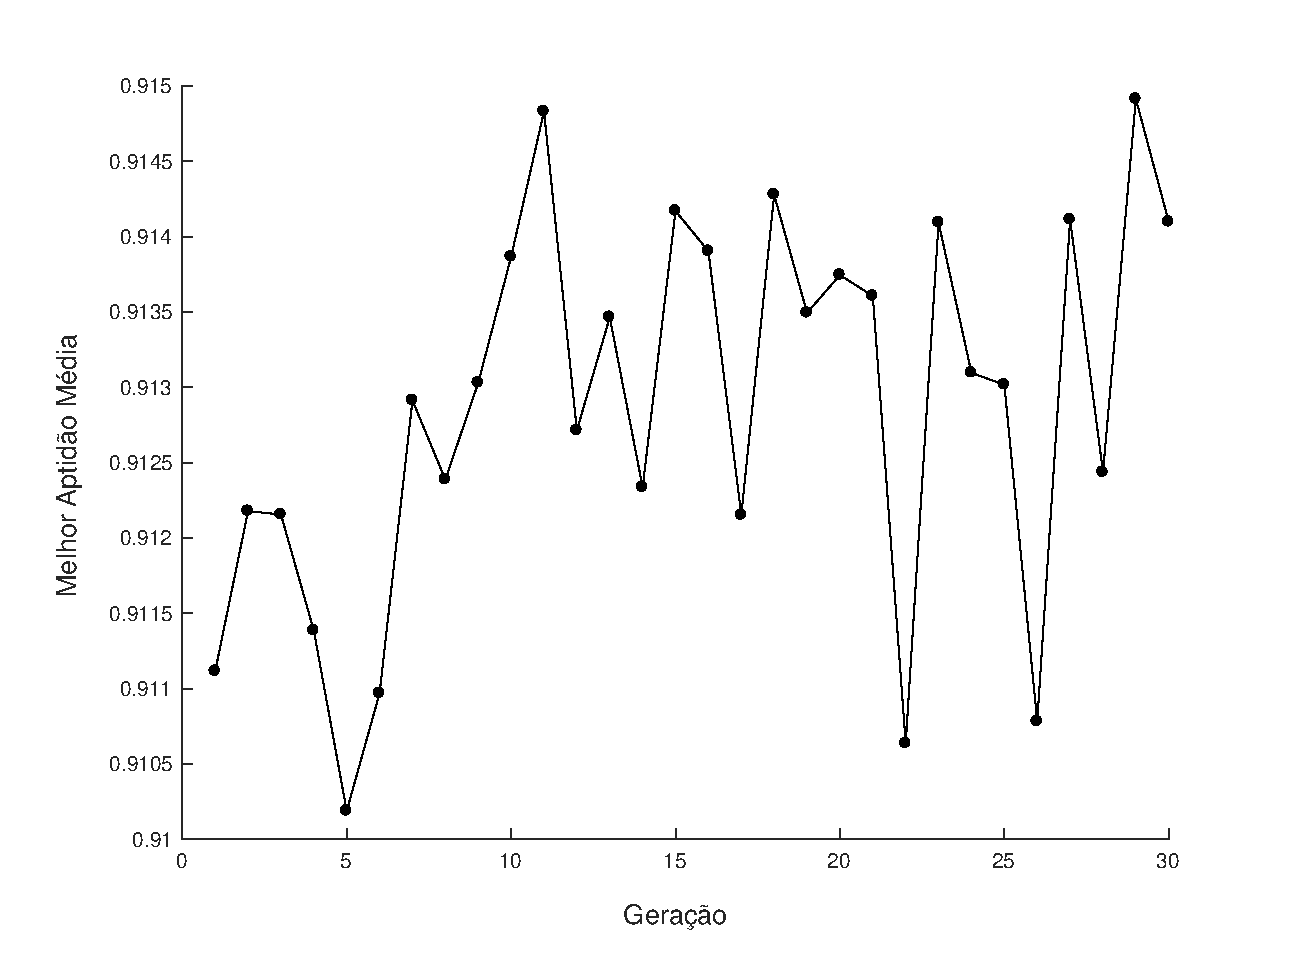
\includegraphics[width=\linewidth]{chapter4/servo.eps}
        \caption{\textit{Servo Motor}}
        \label{fig8:b}
    \end{subfigure}
    \begin{subfigure}[b]{0.5\linewidth}
        \centering
        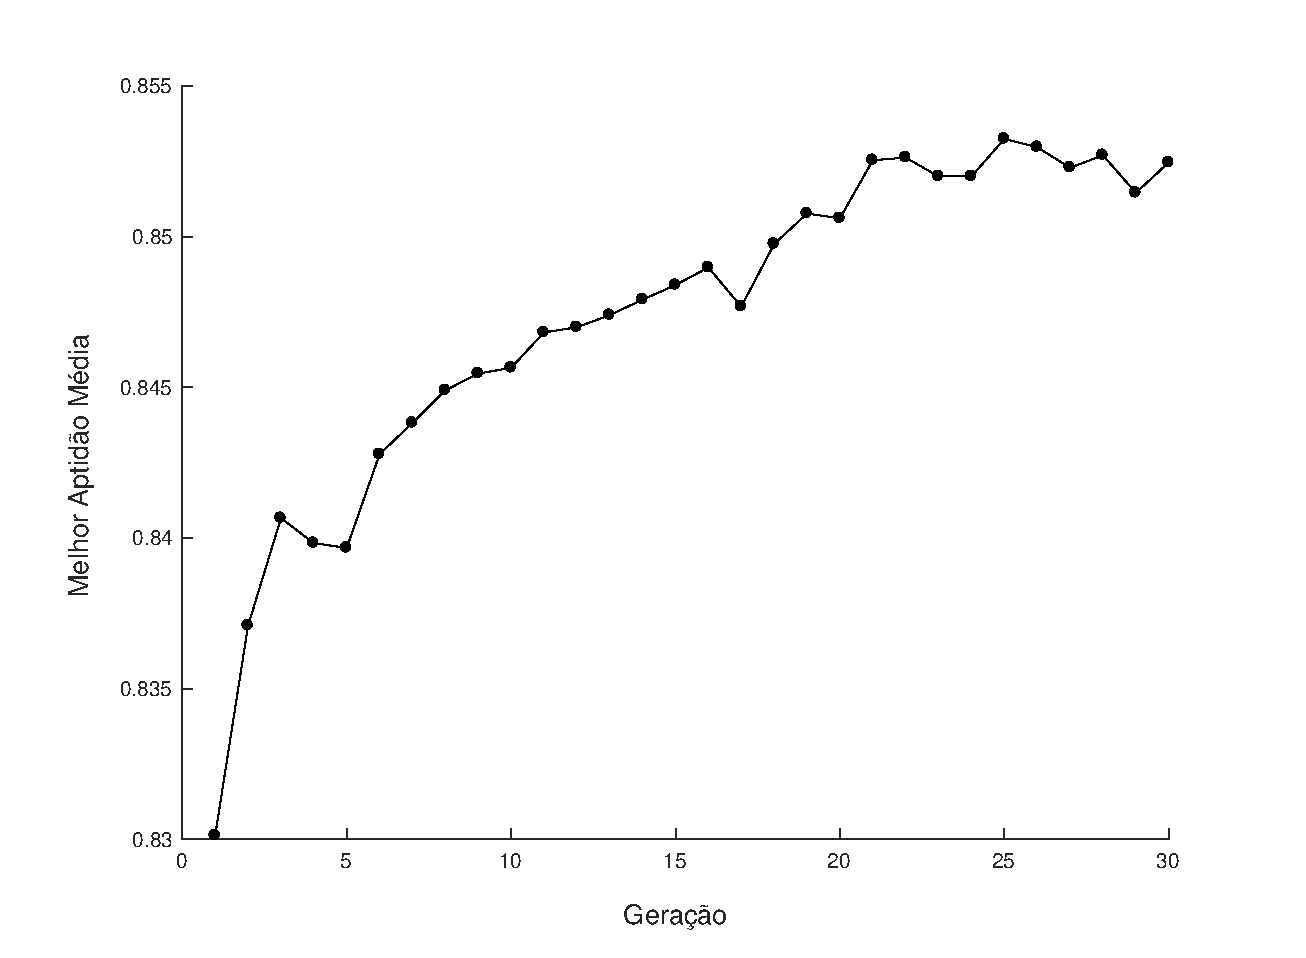
\includegraphics[width=\linewidth]{chapter4/sleep.eps}
        \caption{\textit{Sleep}}
        \label{fig8:c}
    \end{subfigure}%%
    \begin{subfigure}[b]{0.5\linewidth}
        \centering
        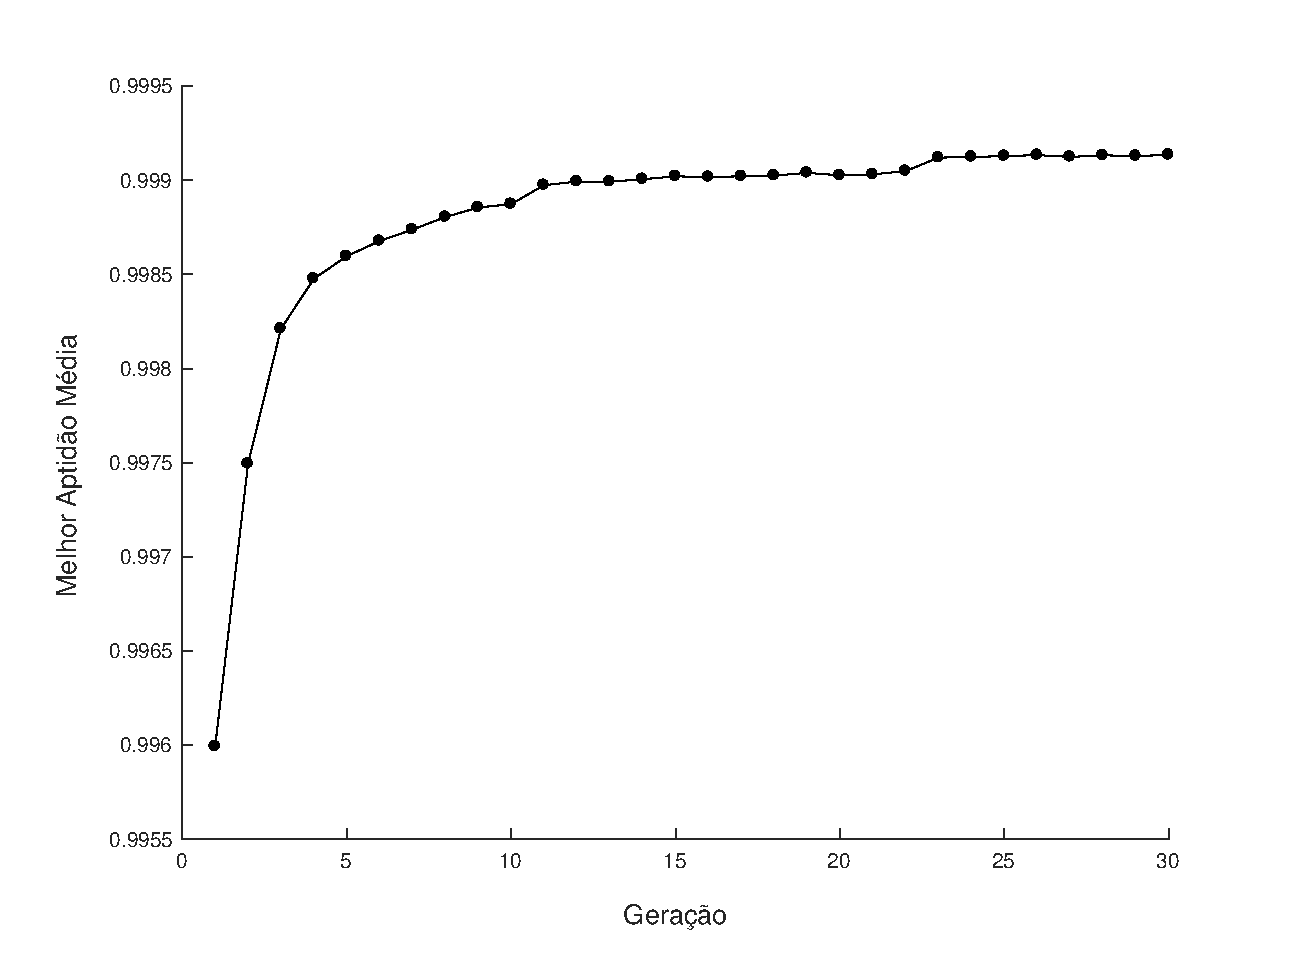
\includegraphics[width=\linewidth]{chapter4/spiritwt.eps}
        \caption{\textit{Spirituos Liquors}}
        \label{fig8:f}
    \end{subfigure}
    \begin{subfigure}[b]{0.5\linewidth}
        \centering
        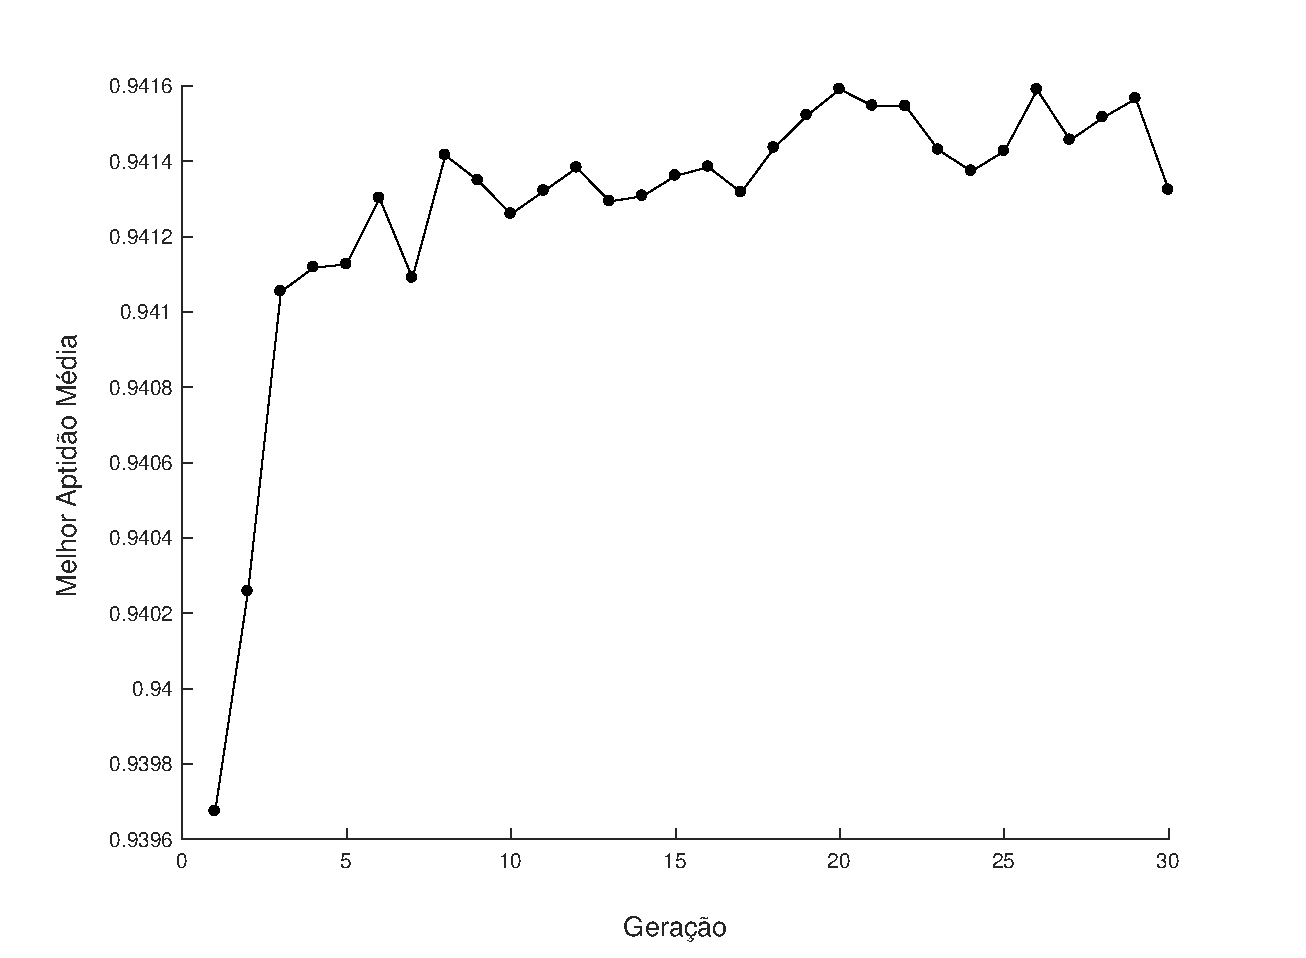
\includegraphics[width=\linewidth]{chapter4/stocks.eps}
        \caption{\textit{Stock Prices}}
        \label{fig8:d}
    \end{subfigure}%%
    \begin{subfigure}[b]{0.5\linewidth}
        \centering
        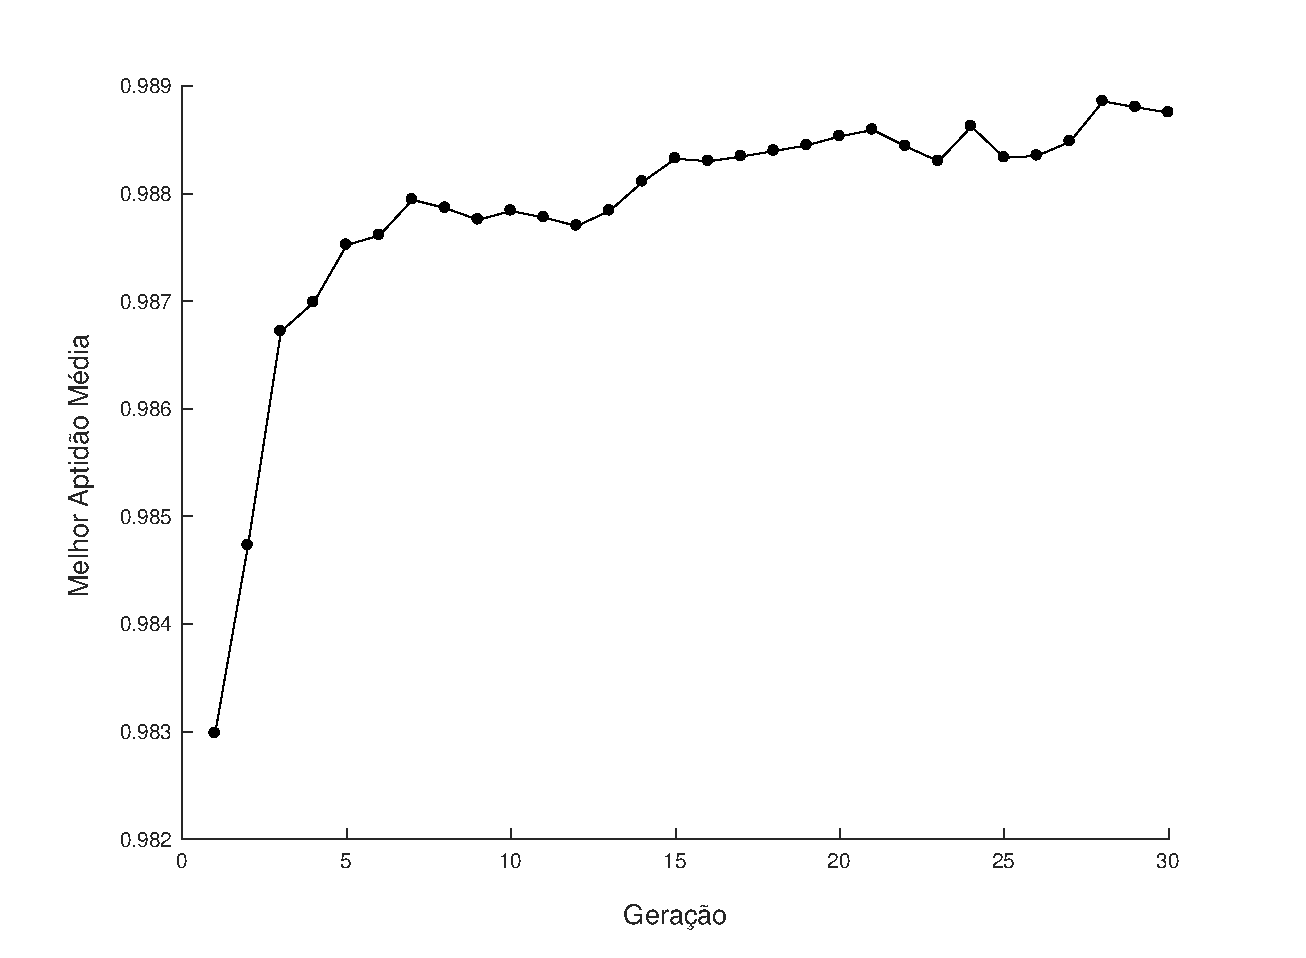
\includegraphics[width=\linewidth]{chapter4/yacht.eps}
        \caption{\textit{Yacht Hydrodynamics}}
        \label{fig8:e}
    \end{subfigure}
    \centering \makebox[\width]{Fonte: Autor.}
\end{figure}

\begin{landscape}
    \begin{table}
        \centering
        \caption{RMSE e tempo total (treinamento e teste) médios de todas as técnicas sobre os conjuntos de dados reais.}
        \label{tab:results-rmse}
        \begin{tabular}{l|l|c@{\hskip 5pt}c@{\hskip 5pt}c@{\hskip 5pt}c@{\hskip 5pt}c@{\hskip 5pt}c}
            \toprule
            \multicolumn{2}{l}{\textbf{Conjunto de dados}} & \textbf{GKR} & \textbf{SVR/LIN} & \textbf{SVR/RBF} & \textbf{SVR/POL} & \textbf{MLP} & \textbf{RBF} \\
            \midrule
            \multirow{2}{*}{APOL}   & RMSE & $0.1360 \pm 0.0331$ & $\textbf{0.1246} \pm \textbf{0.0264}$ & $0.1294 \pm 0.0248$ & $0.1578 \pm 0.0498$ & $0.1612 \pm 0.0367$ & $0.1913 \pm 0.0649$ \\
                                    & Tempo (s) & $469652.30$ & $249.06$ & $20191.93$ & $37230.50$ & $17948.53$ & $16839.90$ \\
            \midrule
            \multirow{2}{*}{AMPG}   & RMSE & $0.0748 \pm 0.0089$ & $0.0945 \pm 0.0095$ & $\textbf{0.0727} \pm \textbf{0.0091}$ & $0.0762 \pm 0.0099$ & $0.0959 \pm 0.0073$ & $0.2663 \pm 0.0943$ \\
                                    & Tempo (s) & $601425.77$ & $172.23$ & $18398.40$ & $54114.76$ & $18983.53$ & $218956.50$ \\
            \midrule
            \multirow{2}{*}{APRI}   & RMSE & $\textbf{0.0773} \pm \textbf{0.0232}$ & $0.0901 \pm 0.0185$ & $0.0909 \pm 0.0244$ & $0.0812 \pm 0.0185$ & $0.0963 \pm 0.0149$ & $0.0838 \pm 0.0215$ \\
                                    & Tempo (s) & $299075.60$ & $66.63$ & $11864.96$ & $25424.90$ & $11142.83$ & $15466.16$ \\
            \midrule
            \multirow{2}{*}{BHOU}   & RMSE & $\textbf{0.0705} \pm \textbf{0.0134}$ & $0.1096 \pm 0.0152$ & $0.0929 \pm 0.0179$ & $0.0766 \pm 0.0178$ & $0.1114 \pm 0.0110$ & $0.1066 \pm 0.0213$ \\
                                    & Tempo (s) & $381618.90$ & $70.30$ & $24801.80$ & $82692.87$ & $12411.93$ & $107767.97$ \\
            \midrule
            \multirow{2}{*}{CHAR}   & RMSE & $0.0524 \pm 0.0373$ & $0.0588 \pm 0.0322$ & $0.0693 \pm 0.0433$ & $0.0575 \pm 0.0346$ & $0.0694 \pm 0.0216$ & $\textbf{0.0514} \pm \textbf{0.0232}$ \\
                                    & Tempo (s) & $296862.33$ & $63.70$ & $11621.53$ & $24732.67$ & $10452.77$ & $6508.03$ \\
            \midrule
            \multirow{2}{*}{DIAB}   & RMSE & $0.1904 \pm 0.0570$ & $\textbf{0.1681} \pm \textbf{0.0383}$ & $0.1748 \pm 0.0402$ & $0.1742 \pm 0.0395$ & $0.1738 \pm 0.0464$ & $1.4968 \pm 1.9164$ \\
                                    & Tempo (s) & $430191.17$ & $198.07$ & $26038.67$ & $42552.50$ & $18907.00$ & $20731.70$ \\
            \midrule
            \multirow{2}{*}{SERV}   & RMSE & $\textbf{0.0870} \pm \textbf{0.0177}$ & $0.1911 \pm 0.0376$ & $0.1212 \pm 0.0422$ & $0.0926 \pm 0.0295$ & $0.1662 \pm 0.0179$ & $0.1759 \pm 0.1761$ \\
                                    & Tempo (s) & $583503.90$ & $109.13$ & $20633.30$ & $48024.23$ & $17055.33$ & $56257.00$ \\
            \midrule
            \multirow{2}{*}{SLEE}   & RMSE & $0.1896 \pm 0.0507$ & $0.1822 \pm 0.0315$ & $0.1922 \pm 0.0298$ & $\textbf{0.1782} \pm \textbf{0.0333}$ & $0.2629 \pm 0.1579$ & $18.7917 \pm 44.4962$ \\
                                    & Tempo (s) & $397893.73$ & $178.13$ & $20251.43$ & $39408.90$ & $18640.97$ & $17441.23$ \\
            \midrule
            \multirow{2}{*}{SPIR}   & RMSE & $\textbf{0.0008} \pm \textbf{0.0005}$ & $0.0496 \pm 0.0039$ & $0.0180 \pm 0.0030$ & $0.0192 \pm 0.0011$ & $0.0667 \pm 0.0020$ & $0.0244 \pm 0.0029$ \\
                                    & Tempo (s) & $982922.37$ & $191.03$ & $17347.23$ & $44298.63$ & $80656.60$ & $9519.30$ \\
            \midrule
            \multirow{2}{*}{STPR}   & RMSE & $\textbf{0.0262} \pm \textbf{0.0015}$ & $0.0847 \pm 0.0057$ & $0.0277 \pm 0.0020$ & $0.0311 \pm 0.0018$ & $0.0899 \pm 0.0045$ & $0.0361 \pm 0.0024$ \\
                                    & Tempo (s) & $671482.47$ & $140.93$ & $13440.30$ & $382495.63$ & $17045.13$ & $64897.67$ \\
            \midrule
            \multirow{2}{*}{YAHY}   & RMSE & $\textbf{0.0098} \pm \textbf{0.0020}$ & $0.1714 \pm 0.0221$ & $0.1181 \pm 0.0194$ & $0.0202 \pm 0.0030$ & $0.1483 \pm 0.00103$ & $0.0314 \pm 0.0074$ \\
                                    & Tempo (s) & $541210.30$ & $322.77$ & $38270.83$ & $169372.80$ & $26527.77$ & $11744.00$ \\
            \midrule
            \multirow{2}{*}{WPBC}   & RMSE & $\textbf{0.2558} \pm \textbf{0.0170}$ & $0.2629 \pm 0.0235$ & $0.2636 \pm 0.0250$ & $0.3335 \pm 0.0432$ & $0.2823 \pm 0.0300$ & $0.5227 \pm 0.1855$ \\
                                    & Tempo (s) & $467865.40$ & $208.70$ & $24975.87$ & $48350.63$ & $37693.87$ & $71121.93$ \\
            \bottomrule
        \end{tabular}
        \begin{center}
            \makebox[\width]{Fonte: Autor.}
        \end{center}
    \end{table}
\end{landscape}
